\toftagthis{folk}
\song{Dajána}{Paul Anka / Zdeněk Borovec}{30pt}{1}{
\verse{1}{}\C{}Lidé o ní \Am{}říkají,\F{} že je v lásce \G[7]{}nevěrná,\\
ona zatím potají jediného v mysli má,\\
na toho, kdo klid jí vzal, dnem i nocí čeká dál,\\
krásná, bláhová Dajána. 

\verse{2}{}Ten, kdo jí klid navždy vzal, odešel si bůhvíkam,\\
Dajána má v srdci žal, žije marným vzpomínkám,\\
předstírá-li ve dne smích, pláče v nocích bezesných,\\
krásná, bláhová Da\C{}jána\C[7]{}. 

\verse{*}{}\F{}Srdce, které \Fm{}zasteklo si, \C{}s úsměvem teď \C[7]{}žal svůj nosí,\\
\F{}stále čeká, \Fm{}čeká dál\ldots{}Ó\G{}o óo ó\G[7]{}ooo oooo 

\verse{3}{}Ospalá jde ulicí, nezbaví se lásky pout,\\
sny, jež voní skořicí, sny, jež nelze obejmout,\\
navždy bude sama snít, nenalezne nikdy klid,\\
krásná, bláhová Dajána.\\
}


\toftagthis{nohavica}
\song{Darmoděj}{Jaromír Nohavica}{25pt}{1}{
\vskip 10pt
\crdheight=2.9ex
\verse{1}{}\Am{}Šel včera městem \Em{}muž a šel po hlavní \Am{}třídě,\Em{}\\
\Am{}šel včera městem \Em{}muž a já ho z okna \Am{}viděl,\Em{}\\
\C{}na flétnu chorál \G{}hrál, znělo to jako \Am{}zvon\\
a byl v tom všechen \Em{}žal, ten krásný dlouhý \F{}tón,\\
a já jsem náhle \Ds[dim]{}věděl: Ano, to je \E[7]{}on, to je \Am{}on. 

\verse{2}{}Vyběh' jsem do ulic jen v noční košili,\\
v odpadcích z popelnic krysy se honily\\
a v teplých postelích lásky i nelásky\\
tiše se vrtěly rodinné obrázky,\\
a já chtěl odpověď na svoje otázky, otázky. 

\chorus{}\Am{}Na na \Em{}na\ldots{}\C{} \hskip 1em \G{} \hskip 1em \Am{} \hskip 2em \F{} \hskip 1em \Ds[dim]{} \hskip 3em \E[7]{} \hskip 2.5em \CHORD{(2$\times$)}{}

\verse{3}{}Dohnal jsem toho muže a chytl za kabát,\\
měl kabát z hadí kůže, šel z něho divný chlad,\\
a on se otočil a oči plné vran\\
a jizvy u očí, celý byl pobodán,\\
a já jsem náhle věděl, kdo je onen pán, onen pán. 

\verse{4}{}Celý se strachem chvěl, když jsem tak k němu došel,\\
a v ústech flétnu měl od Hieronyma Bosche,\\
stál měsíc nad domy jak čírka ve vodě,\\
jak moje svědomí, když zvrací v záchodě,\\
a já jsem náhle věděl: to je Darmoděj, můj Darmoděj. 

\chorus{}Můj Darmoděj, vagabund osudů a lásek,\\
jenž prochází všemi sny, ale dnům vyhýbá se,\\
můj Darmoděj, krásné zlo, jed má pod jazykem,\\
když prodává po domech jehly se slovníkem. 

\verse{5}{}Šel včera městem muž, podomní obchodník,\\
šel, ale nejde už, krev skápla na chodník,\\
já jeho flétnu vzal a zněla jako zvon\\
a byl v tom všechen žal, ten krásný dlouhý tón,\\
a já jsem náhle věděl: ano, já jsem on, já jsem\ldots{}  

\chorus{}Váš Darmoděj, vagabund osudů a lásek,\\
jenž prochází všemi sny, ale dnům vyhýbá se,\\
váš Darmoděj, krásné zlo, jed mám pod jazykem,\\
když prodávám po domech jehly se slovníkem.\\
\noexport{
~\\
\textbf{Intro:}\\
\vskip -15pt
\begin{figure}[h!]
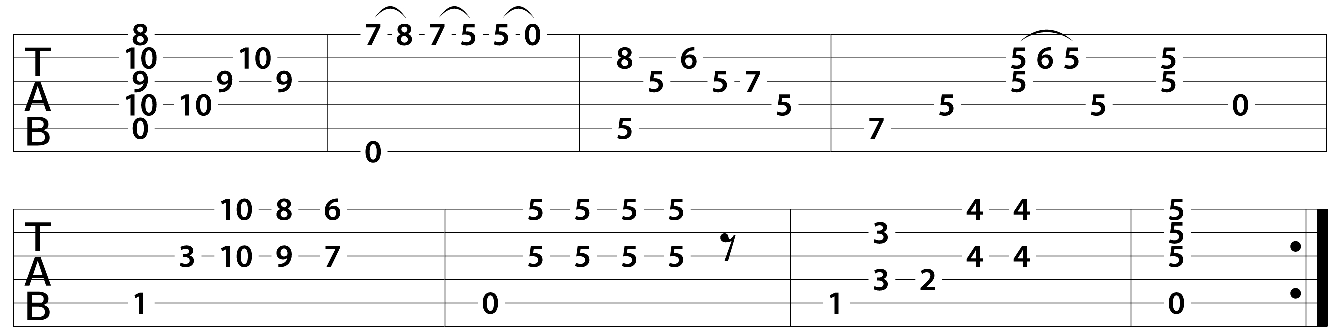
\includegraphics[width=365pt, height=100pt ]{res/darmodej.pdf}
\end{figure}
}
}


\toftagthis{vw}
\song{David a goliáš}{J. Ježek / V+W}{10pt}{0.99}{
\crdheight=2.3ex
\verse{1}{}\C{}Lidi na li\Am{}di jsou jako \F{}san\G[7]{}ě, \hskip 1em
\C{}člověk na člo\Am{}věka jako \F{}kat\G[7]{},\\
\C{}podívejte \A[7]{}se na ně, \Dm{}musíte \G[7]{}naří\C{}kat.\H[7]{}\\
\Em{}Obr do pidimužíka \A{}myd\H[7]{}lí, \hskip 0.8em \Em{}domnívaje se, že vyhra\A{}je,\H[7]{}\\
\G{}klidně \Em{}seďme \Am{}na žid\D[7]{}li, \hskip 0.8em \G{}čtěme bibli, \G[7]{}tam to všechno je.

\verse{2}{}\C{}Samuelo\Am{}va kniha nám \Dm[7]{}poví - \G[7]{}dá,\\
\C{}jak na žida \Am{}přišla veli\Dm[7]{}ká bí - \G[7]{}da,\\
\C{}jak ti bídní \Am{}Filištíni \F{}válku vést ne\Fm{}byli líní,\\
\C{}až potkali \Ab[7]{}Davi\G[7]{}da. 

\verse{3}{}\C{}David šel do \Am{}války volky, \Dm[7]{}nevol - \G[7]{}ky,\\
\C{}z velké dálky \Am{}nesl bratrům \Dm[7]{}homol - \G[7]{}ky,\\
\C{}v pochodu se \Am{}cvičil v hodu, \F{}dal si pro strý\Fm{}čka Příhodu\\
\C{}tři šutry do \G[7]{}tobol\C{}ky.

\verse{*}{}\uv{Hej, \Ab{}hej, kam se \C{}valej, vždyť jsou \D[7]{}malej!}\\
Takhle \G[7]{}Goliáš ho \E[7]{}provokuje,  \Dm[7]{}David slušně \G[7]{}salutuje.

\verse{4}{}\C{}Když mu \Am{}ale obr plivnul \Dm[7]{}do očí,\G[7]{}\\
\C{}David se o\Am{}točí, prakem \Dm[7]{}zato - \G[7]{}čí,\\
\C{}když začínáš, \Am{}no tak tu máš, \F{}byl jsi velkej \Fm{}já měl kuráž\\
\C{}a jakej byl \D[7]{}Go - \G[7]{}li - \C{}áš!

~\\
\hskip 5em \emph{(pokračování dle verze z roku 1952)}\\
\leftskip 45pt
\rec{Vcelku, to co jsme dnes slyšeli, to není nic nového,\\
to je stará příhoda, ale zajímavá věc,\\
ono to má pokračování:}


\textbf{\textsf{Akordy jako ve 2.,3.,*.,4.}}\\
\verse{5}{}Jestli masy nebudou dost masívní\\
a zůstanou ještě pár let pasívní,\\
stanou se pak tyto masy asi už na věčné časy\\
radioaktívní.\\
\verse{6}{}Víte, co je zapotřebí nápadů,\\
jak se zbavit nukleárních odpadů,\\
víte-li, co zla natropí bez kontroly izotopy\\
tisíc let po dopadu.\\
\verse{*}{}Ba jó, my to víme a tvrdíme,\\
mějme hlavy v písku, jako pštrosi,\\
nejvejš nám to spálí šosy.\\
\verse{7}{}Jenže lidem nejde jenom o šosy,\\
ale o krk a o značný obnosy,\\
a proto by měly masy, říct své slovo všemi hlasy,\\
dřív než nás smrt pokosí!\\
}


\toftagthis{raduza}
\song{De nîmes}{Radůza}{50pt}{1}{
\verse{1}\Am{}Očima uhla \Dm{}jsem \Em{}a nebylo to stu\Am{}dem.\\
\Am{}Peřina pohla \Dm{}se, \hskip 1em \G{}nějak už \Am{}bude.\\
Lino je studený, ponožky a pak triko.\\
A kabát přes denim a nic a ticho.

\verse{*}Cette \Am{}chanson n’a jamais été chantée\\
\Dm{}comme il faut, c’est ça\\
Mais \G{}si tu veux, nous \Em{}tous les deux\\
pou\Am{}vons le faire, comme ça

La \Am{}tranquillité, c’est ce qu’on cherche on\\
\Dm{}dit: »Puisse-t-elle venir!«\\
On \G{}dit que tout est \Em{}dificile\\
mais, \Am{}qu’ est-ce que ça veut dire

\chorus{}\Am{}Zouvám si pár \Dm{}těžkejch bot,\\
jsi \G{}ve ves\Em{}míru můj \Am{}pevnej bod.\\
A sukně kasám, je blízko brod\\
a pryč je, co kdo zbod.

\verse{2}Jen hlesnu od dveří:
\uv{Víš, nelhala jsem dosud.\\
A jestli nevěříš,
zkus špičku nosu.}\\
Okna jsou zamžený,
nádobí škopek plnej,\\
mám hrdlo stažený,
hajej a nynej.\\
\verse{*}Cette chanson \dots\\
\chorus{}Zouvám si pár těžkejch bot \dots 

\verse{3}Očima uhla jsem
a nebylo to studem.\\
Poznal jsi po hlase
jak mi teď bude.\\
Lino je studený,
pod kafem stůl se kejvá.\\
Un souvenir de Nîmes,
tak už to bejvá.\\
\verse{*}Cette chanson \dots\\
\chorus{}Zouvám si pár těžkejch bot \dots\\
}


\toftagthis{olympic}
\song{Dej mi víc své lásky}{Olympic}{30pt}{0.89}{
\verse{1}{}\Em{}Vymyslel jsem spoustu nápadů, a\G{}úú\\
co \Em{}podporujou hloupou nála\D{}du, a\H[7]{}úú,\\
\Em{}hodit klíče do kanálu, \A{}sjet po zadku \Am{}holou skálu,\\
\Em{}v noci chodit \H[7]{}strašit do hra\Em{}du.

\verse{2}{}Dám si dvoje housle pod bradu, aúú,\\
v bíle plachtě chodím pozadu, aúú,\\
úplně melancholicky, s citem pro věc, jako vždycky,\\
vyrábím tu hradní záhadu, a\D[7]{}úú.

\vskip -1ex
\chorus{} \G{}Má drahá, dej mi víc, \H[7]{}má drahá, dej mi víc,\\
\Em{}má drahá, \C{}dej mi víc své \G{}lásky, a\D[7]{}úú.\\
\G{}Já nechci skoro nic, \H[7]{}já nechci skoro nic,\\
\Em{}já chci jen \C{}pohladit tvé \G{}vlásky, a\H[7]{}úú!

\verse{3}{}Nejlepší z těch divnejch nápadů, aúú,\\
mi dokonale zvednul náladu, aúú,\\
natrhám ti sedmikrásky, tebe celou s tvými vlásky\\
zamknu si na sedm západů, aúú.\\
\textbf{R:}

\verse{4. = 3}{}\ldots{}+ aúú, aúú, aúú, aúú. 
}

\toftagthis{nohavica}
\song{Divoké koně}{Jaromír Nohavica}{15pt}{1}{
\capo{5}
\verse{1}\revrpt{} \Em{}Já viděl divoké koně, \G{}běželi \Am{}soumra\Em{}kem, \rpt{}\\
\Am{}vzduch \Em{}těžký \Am{}byl a divně \Em{}voněl\Ds[dim]{} \hskip 1em tabá\C{}kem,\\
\Am{}vzduch \Em{}těžký \Am{}byl a divně \Em{}voněl \H[7]{}tabá\Em{}kem.

\vskip -1ex
\verse{2}\revrpt{} Běželi, běželi, bez uzdy a sedla, krajinou řek a hor, \rpt{}\\
\revrpt{} sper to čert, jaká touha je to vedla za obzor. \rpt{}

\vskip -2ex
\verse{3}\revrpt{} Snad vesmír nad vesmírem, snad lístek na věčnost, \rpt{}\\
\revrpt{} naše touho ještě neumírej, sil máme dost. \rpt{}

\vskip -2ex
\verse{4}\revrpt{} V nozdrách sládne zápach klisen na břehu jezera, \rpt{}\\
\revrpt{} milování je divoká píseň večera. \rpt{}

\vskip -2ex
\verse{5}\revrpt{} Stébla trávy sklání hlavu, staví se do šiku, \rpt{}\\
\revrpt{} král s dvořany přijíždí na popravu zbojníků. \rpt{}

\vskip -2ex
\verse{6}\revrpt{} \scalebox{0.97}[1]{\textls[-40]{Chtěl bych jak divoký kůň běžet běžet, nemyslet na návrat,\,}}\rpt{}\\
\revrpt{} s koňskými handlíři vyrazit dveře, to bych rád. \rpt{}

\vskip -1ex
Já viděl divoké koně!\\
\vskip 12pt
\begin{figure}[h!]
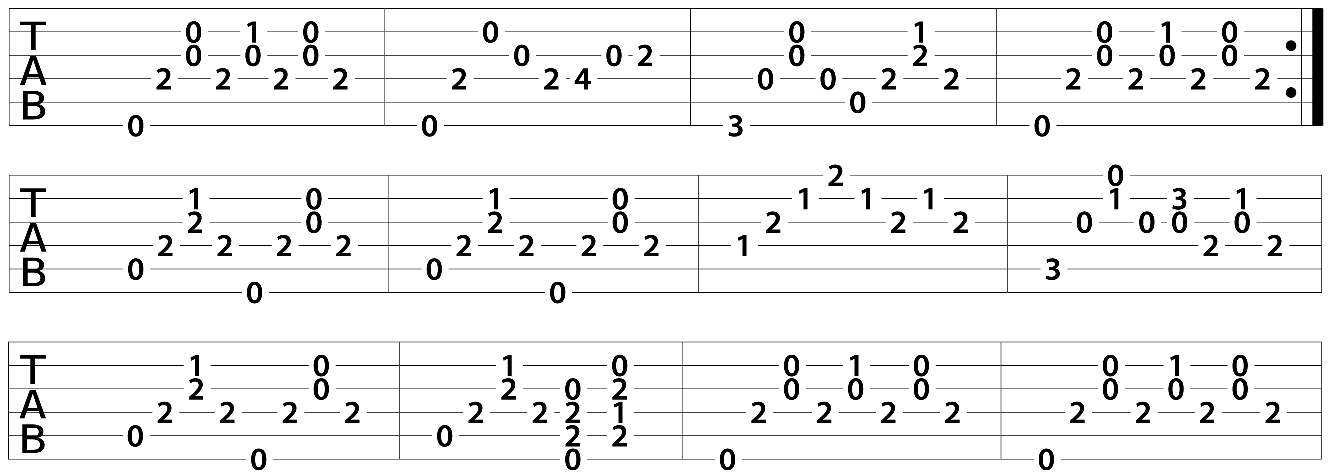
\includegraphics[width=365pt ]{res/divoke.pdf}
\end{figure}
\vskip -40pt
}


\toftagthis{hapka}
\song{Dívám se, dívám}{Petr Hapka / Michal Horáček}{12pt}{1}{
\verse{1}\D{}Dívám se, dívám a ty \A{}spíš, matně se leskne malý \G{}kříž.\\
Stoupá a klesá tvoje hruď\\
a já si říkám: \uv{Bůh jen \D{}suď, Bůh jen \A{}suď.}

\verse{2}Zdali, až jednou blýskne se a vítr liják přinese,\\
vezmeš mě k teplu pod svůj plášť.\\
Jestli to pro mě uděláš?

\verse{*}\D{}Když budu sedět nehnu\A{}tě a zase \D[maj]{}znovu zklamu \E{}tě\\
svým dojmem, že jsem na pouš\D{}ti\\
a že mě štěstí opouš\A{}tí,\hskip 1em \E{}

\verse{3}\D{}Zeptáš se: \uv{Kam jsi oči \A{}dal? Tvá šťastná hvězda svítí \G{}dál!\\
Jdi za ní, já tu držím stráž\ldots}\\
\chorus{}\revrpt{} \D{}Tak se \G[maj]{}ptám, jestli to \A{}uděláš, \rpt{}\\
pro mě \D{}uděláš.

\verse{4}\F{}Co když se těžce zadlu\C{}žím? I ten kříž prodáš? Co já \Bb{}vím.\\
Když mě mé masky unaví,\\
stáhneš mě k sobě do trá\F{}vy, do trá\C{}vy.

\verse{5}\uv{A klidně řekneš hroznou lež: Na svoje léta hezkej seš.\\
Před sebou ještě všechno máš\ldots}\\
Jestli to pro mě uděláš?

\verse{*}\F{}Co když mě zapřou přáte\C{}lé a budu s \F[maj]{}cejchem na \G{}čele\\
podroben strašné žalo\F{}bě? Vzkážeš mi: \uv{Stojím při to\C{}bě!\\
Jen při to\G{}bě.

\verse{6}Jediná vždycky budu stát i když ti celý svět dá mat.\\
Věřím ti všecko. Braň se, snaž\ldots}\\
\chorus{}\revrpt{} \F{}Jen se \Bb[maj]{}ptám, zda to \C{}uděláš. \rpt{}\\
Pro mě udě\F{}láš.

\verse{7}\D{}Stou\CHORD{\ldots}{}pá a klesá tvoje hruď, tak spolehlivě jako rtuť,\\
na teploměru našich dní,\\
ráno svět zuby vycení, vycení.

\verse{8}A mně se mnohé nezdaří, ale tvé prsty po tváři\\
mi zvolna přejdou, každý zvlášť.\\
\chorus{}Vím, že to pro mě uděláš.\\
Já vím, že to pro mě uděláš.\\
Všechno uděláš.
}


\toftagthis{brichta}
\song{\textls[-10]{Dívka s perlami ve vlasech}}{Aleš Brichta}{60pt}{0.9}{
\setlength{\parskip}{1ex} % vertical space between paragraphs
\verse{1}{}\Em{}Zas mě tu \D{}máš, ně\Am{}jak se \Em{}mračíš,\\
vybledlej smích už ve dveřích.\\
S čelenkou perel svatozář ztrácíš,\\
kolik se platí za vláčnej hřích.

\chorusAlt{R1:}{-29pt}No tak lás\G{}ko, co \D{}chceš mi říct,\\
\Am{}máš už perly, mož\Em{}ná i víc,\\
lásko, na co se ptáš, svíčku zhasínáš.\\
Nemám, lásko, co bych ti dal,\\
chtělas všechno, nebyl jsem král,\\
lásko, na co se ptáš, perly ve vlasech máš.

\verse{2}{}Tvý horky rty, víc radši ne,\\
nejsou už mý, nejsi má Cher.\\
Něco snad chápu, to ne, to ne,\\
bolí to, hořím, jak černej thér.

\chorusAlt{R2:}{-30pt}No tak lásko, kdo mi tě vzal,\\
komus dala, tělo i duši,\\
lásko, na co je pláč, když to skončit má.\\
Vždyť už, lásko, svý perly máš,\\
tak proč padaj', měněj se v slzy,\\
lásko, na co je pláč, perly ve vlasech máš.

\verse{3}{}Chtěla jsi víc pro svoje touhy,\\
já, chudej princ, mám jen, co mám.\\
Co vlastně zbývá, jen slzy pouhý,\\
ze svatebních zvonů, z nebeskejch bran.\\
\textbf{R2: + R1:}
}


\toftagthis{chinaski}
\song{Dlouhej kouř}{Chinaski}{25pt}{1}{
\verse{1}\D{}Když budeš hodná, naučím tě \C{}číst, naučím tě \G{}číst\\
mezi řádky.\\
To pokušení znáš, tak zapomeň cestu zpátky.\\
Hmm\ldots cestu zpátky.\\
Naše noc je mladá, vane jižní vítr,\\
papírový křídla vzduchem víří.\\
Řekni, co bys ráda, než nám ráno plány zkříží.

\verse{*}Půjdem nekonečně dlouhou sametově černou tmou.\\
Půjdem nekonečně dlouhou sametově černou\ldots

\chorus{}Vam pam tyda pam, dám si ruce do kapes.\\
vam pam tyda pam, dlouhej kouř a pohoda jazz.\\
vam pam tyda pam, neštěkne po mě ani pes.\\
padám a nevím kam, nečekej, že ti zavolám.

\verse{2}Když budeš hodná, moje hodná holka,\\
ukážu ti všechny svoje tajný skrýše.\\
Poletíme vejš, chvíli budem řvát, chvíli budem tiše.\\
Úplně tiše\ldots\\
Vezmu si tě celou, budem se mít rádi\\
a když ne, tak se ti něco zdálo.\\
A když budem chtít, šlápnem na zmizík,\\
všechno bude málo.

\verse{*}Půjdem nekonečně dlouhou\ldots + \textbf{R:}\\
}


\toftagthis{klus}
\song{Do nebe}{Tomáš Klus}{20pt}{1}{
\transposeFiveDown 
\verse{1}Haló, \C{}pane,\G{} vy s \Am{}výhledem na celej svět,\F{}\\
co se \C{}stane,\G{} když \Am{}neumím dát odpo\F{}věď?\\
Snad se \C{}nezlobíte,\G{} snad mi to \Am{}odpustíte,\F{}\\
vždyť \F{}víte, \F{}že chci\ldots

\chorus{}\revrpt{} Do nebe, do nebe, do nebe, do nebe, do nebe,\\
do nebe, do nebe, do nebe, do nebe,\\
do nebe, do nebe, do nebe, do nebe, do nebezpečna. \rpt{}

\verse{2}Haló, pane, nad střechami paneláků,\\
až déšť ustane, až uschnou křídla ptáků,\\
budu relativně štastný, budu žádaný a krásný,\\
budu obdivován v očích půvabných dam, ale sám\\
půjdu\ldots\\
\textbf{R:}

\verse{3}Haló, pane, vy s šedivými vousy,\\
jak poznat nepoznané, jak štěstí nevytrousit,\\ 
jak se nadechnout a zůstat živ a zdráv\\
a jestli jít či plout, to bych taky věděl rád,\\
vždyť chci\ldots\\
\textbf{R:}\\
}

\toftagthis{chinaski}
\song{Dobrák od kosti}{Chinaski}{40pt}{0.95}{
\verse{1}{}\C{}Má milá, \G{}jak ti je, tak \F{}jak ti je?\F{}\\
\C{}Jsem ten, kdo \G{}jednou tvý \F{}tělo zakryje.\Bb{} \hskip 1em \emph{\normalsize \textbf{Fine}}\\
Jsem ten, kdo tě jednou oddělá,\\
potkalas zkrátka kohos neměla.

\verse{2}{}Jsi budoucí krev v mojí posteli.\\
Jsem ten, kdo tě jednou jistojistě zastřelí,\\
jsem ten, kdo ty tvoje krásný oči jednou zatlačí.\\
Jsi moje všechno a mně to nestačí.\\
\chorus{}Je to \C{}vážně silná káva, \G{}pláč a nebo vztek,\\
\F{}nic už s tím nenadě\F{}láš.\\
Nech mě jenom hádat, jak jsi hebká na dotek,\\
krásná a nedospělá. 

\verse{3}{}Víš,všechno má aspoň malý kaz,\\
jsem ten, kdo ti jednou zlomí vaz.\\
Má milá, vždyť mě znáš, jsem dobrák od kosti\\
a ty jsi ta, co mi to jednou všechno odpustí. 

\verse{*}{}\revrpt{} Sejde z očí, sejde z mysli,\\
jenom blázen věří na nesmysly,\\
láska je čaroděj a ticho prý léčí,\\
ale zákon hovoří jasnou řečí. \rpt{}\\
\textbf{R:, R: (kluci) + *. (holky)\\ 1. al Fine }
}


\toftagthis{nohavica}
\song{Dokud se zpívá}{Jaromír Nohavica}{22pt}{1}{
\verse{1}{}\C{}Z Těšína \Em{}vyjíždí \Dm[7]{}vlaky co \F{}čtvrthodi\C{}nu,\Em{} \hskip 2.1em  \Dm[7]{} \hskip 2.8em  \G[7]{}\\
\C{}včera jsem \Em{}nespal a \Dm[7]{}ani dnes \F{}nespoči\C{}nu,\Em{} \hskip 2.1em  \D[7]{} \hskip 2.8em  \G[7]{}\\
\F{}svatý \G{}Medard, můj \C{}patron, ťuká \Am{}si na če\G{}lo, \G{}\\
ale \F{}dokud se \G{}zpívá, \F{}ještě se \G{}neumře\C{}lo. \Em{} \hskip 2.1em  \Dm[7]{} \hskip 2.8em  \G[7]{}

\verse{2}{}Ve stánku koupím si housku a slané tyčky,\\
srdce mám pro lásku a hlavu pro písničky,\\
ze školy dobře vím, co by se dělat mělo,\\
ale dokud se zpívá, ještě se neumřelo. 

\verse{3}{}Do alba jízdenek lepím si další jednu,\\
vyjel jsem před chvílí, konec je v nedohlednu,\\
za oknem míhá se život jak leporelo,\\
ale dokud se zpívá, ještě se neumřelo. 

\verse{4}{}Stokrát jsem prohloupil a stokrát platil draze,\\
houpe to, houpe to na housenkové dráze,\\
i kdyby supi se slítali na mé tělo,\\
tak dokud se zpívá, ještě se neumřelo. 

\verse{5}{}Z Těšína vyjíždí vlaky až na kraj světa,\\
zvedl jsem telefon a ptám se: \uv{Lidi, jste tam?}\\
A z veliké dálky do uší mi zaznělo,\\
\revrpt{} že dokud se zpívá, ještě se neumřelo. \rpt{}\\
}


\toftagthis{kabat}
\song{Ďábel a syn}{Kabát}{25pt}{1}{
\verse{1}{}\Dm{}Sedím a koukám, jak \C{}zvrácenej podzim\\
\Am{}stromům svlíká jejich \G{}šat,\\
poslouchám ptáky a jenom tak kouřím,\\
malinko chce se mi spát.\\
Padá mi hlava, pak cejtím, jak někdo\\
lehce mě za ruku vzal,\\
blázen či voják, jak maškara divná tam \Am{}stál\ldots{}\\
já pozval ho \Dm{}dál 

\verse{2}{}Měl špinavej kabát a v ruce flétnu,\\
oči jak z mrtvejch by vstal,\\
na botách bahno snad celýho světa,\\
tuhletu píseň mi hrál.\\
Tu píseň, co zpívám, a vůbec vám nevím,\\
kde na ni akordy vzal,\\
jak jsem tam seděl a koukal a kouřil, to já\ldots{}\\
teprv ji psal.  

\verse{3}{}Povídá: \uv{Hochu, vracím se z flámu,\\
hráli jsme karty se zdá,\\
partii pokera o budoucí vládu,\\
dík bohu vyhrál jsem já.\\
Já měl z pekla štěstí a nebo pár trumfů\\
v rukávu -- podvod, já vím,\\
chcete mě soudit, tak dejte mě na kříž, jsem váš\ldots{}\\
ďábel a syn.}  

\verse{4}{}Pak pomalu mluvil a ničil mě silou,\\
co od věků v sobě už má,\\
drtil mě pravdou a pouštěl mi žilou,\\
na závěr jen povídá:\\
\uv{Bůh stvořil lásku a žal, taky bolest\\
a já jenom ubohej chtíč,\\
fandím vám lidem, nevím proč nemáš mě rád\ldots{}}\\
já poslal ho pryč.  

\verse{5}{}Sedím a koukám, jak zvrácenej podzim\\
stromům svlíká jejich šat,\\
přemejším o tom, co s náma bude\\
a malinko chce se mi spát.\\
Padá mi hlava, pak cejtim, jak někdo\\
lehce mě za ruku vzal,\\
blázen či voják, jak maškara divná tam stál\ldots{}\\
tak pozvem ho dál.\\
}
